\documentclass[letter]{ourGreenwayBrand}

\headerlabel{Research Brief}

\titletext{Dispatches: Cycling Without Age (CWA1)}
\subtitletext{Dispatches: along the (c)way!}
\authortext{Cody Wang and Francine Harris}
\editedtext{Darnel Harris}
\datetext{August 16, 2025}

\begin{document}
\MakeBrandTitle

\section{Editor's Note}
Editor’s note:In August 2022 we moved our Cycling Without Age\footnote{\url{https://cyclingwithoutage.ca/}}trikes from Rexdale to the Downsview community by way of Jane and Finch. The stories here are earnest and honest first person point of view reflections of our afternoon’s journey from the perspective of one of our summer pilots and Our Greenway’s senior board member. As our travels accelerating micromobility continue, we look forward to making this an ongoing feature.

\textasciitilde{} The Our Greenway Team

\begin{figure}[htbp]
  \centering
  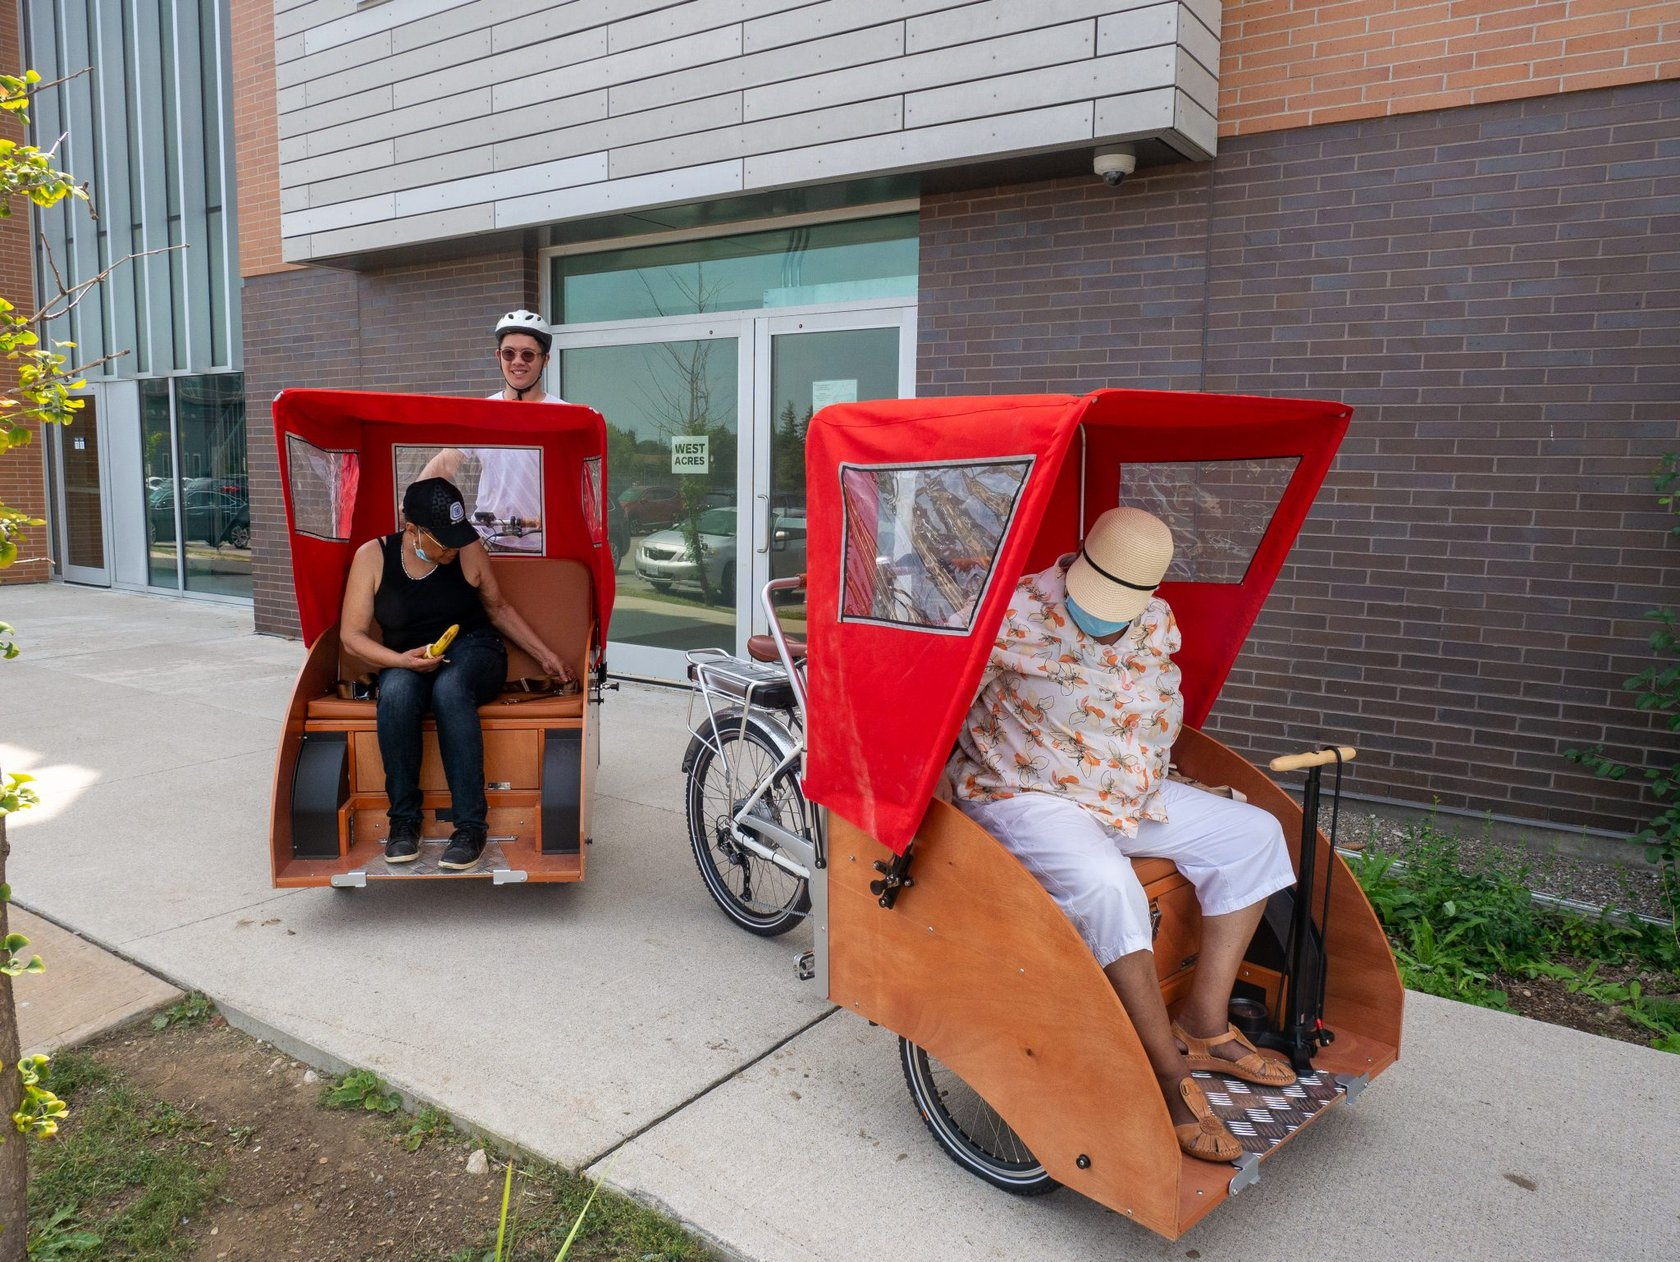
\includegraphics[width=0.7\textwidth]{images/1220468-2048x1538.jpg}
\end{figure}

\section{Cody Wang: “Where’s the Yellow Brick Road?”}
Speaking from my experience being a Trishaw pilot and taking a trip from Rexdale to York University, I will say that for me, if I was summarizing our trip with one word, that word would be ‘counterintuitive’.

First, there were no wayfinding signs or other indicators telling me where to go. I had to rely on following our team lead’s previous experience making the trip himself, but even he had difficulty remembering the route (leading once to a pleasant but lengthy detour).

The hydro corridor section, however, was a pleasant trip. I would say that it is one of the best features of the Northwest Toronto Area. As slower-moving trishaws we did  have to contend with sharing space with faster-moving bikes, scooters, e-bikes, e-scooters and slower-moving pedestrians. The width of the Trishaws also meant that we took up half the paved way.

Heading off the trail and onto Weston Road, we encountered a severe incline. Were it not for the e-assist, it would have been difficult to climb over to Finch Avenue.

\begin{figure}[htbp]
  \centering
  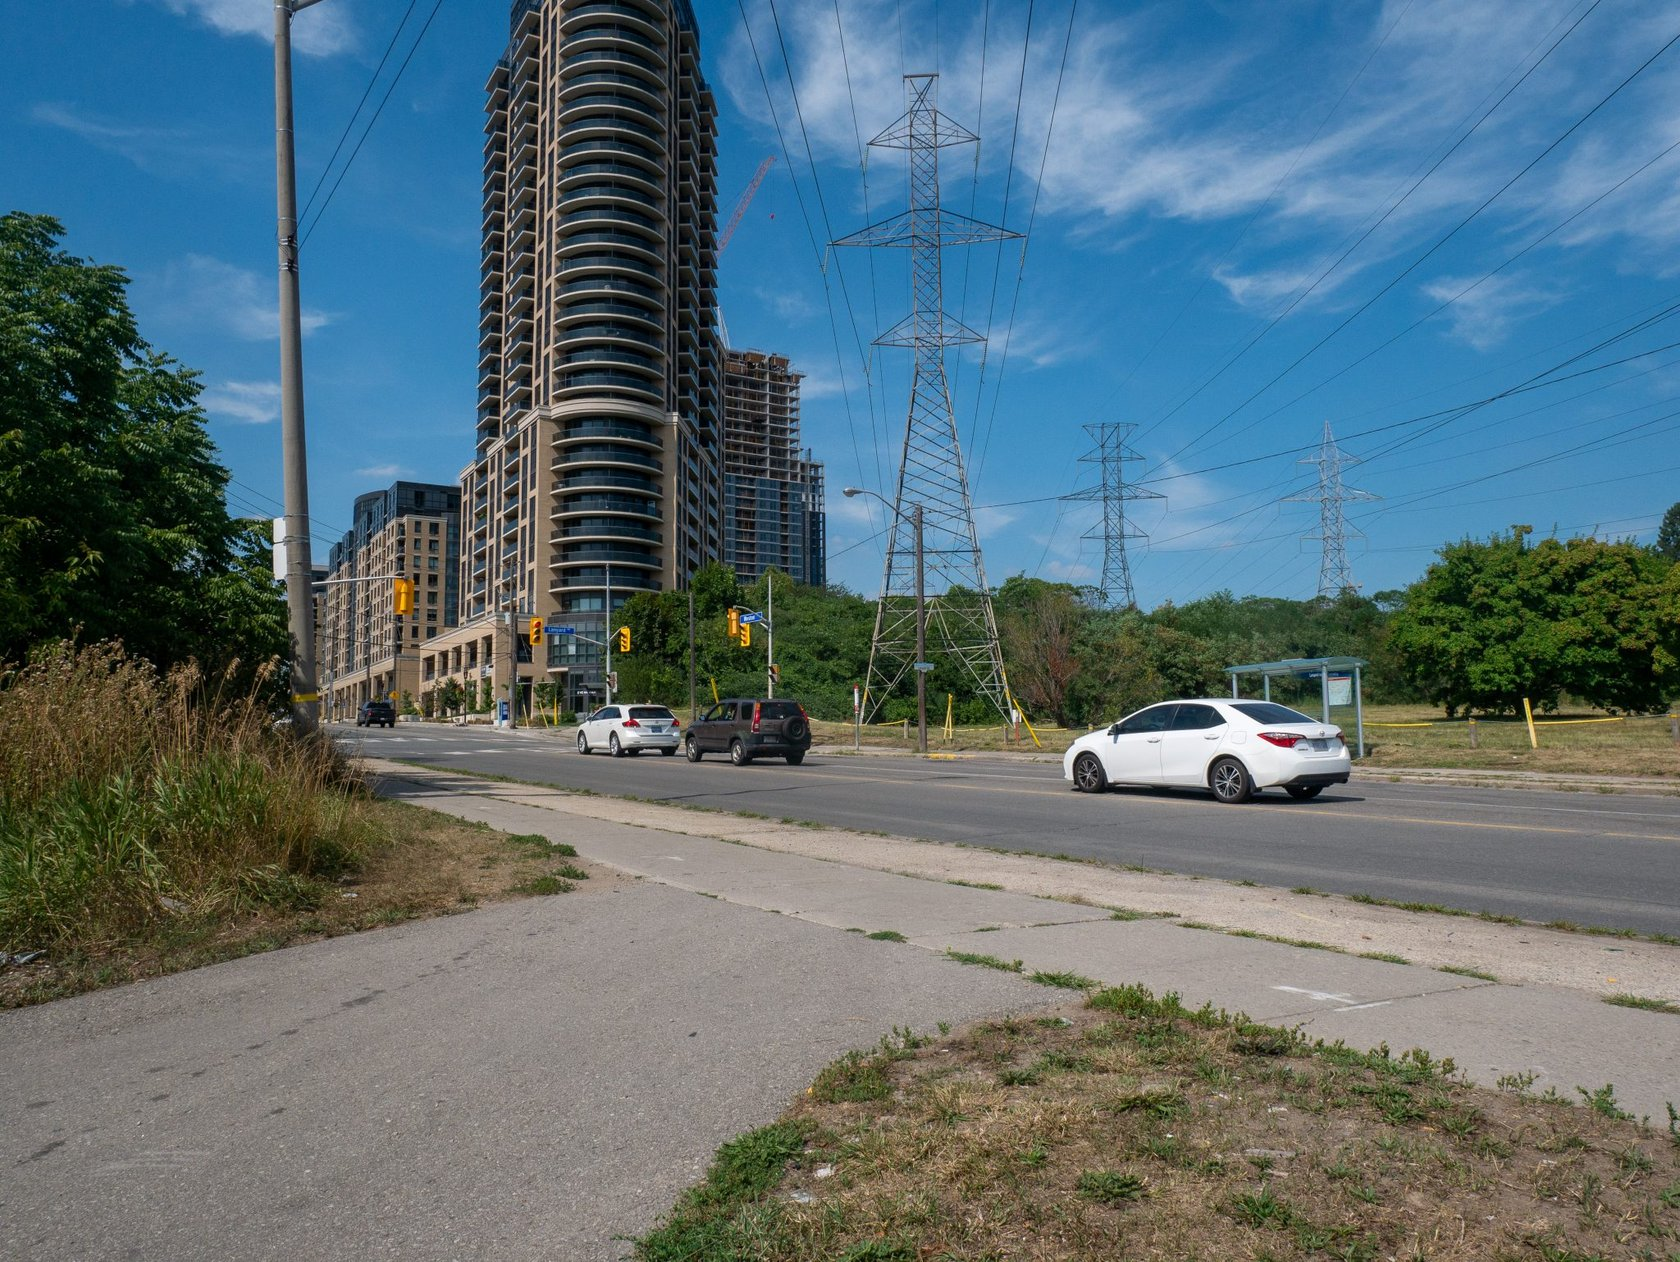
\includegraphics[width=0.7\textwidth]{images/1220590-2048x1538.jpg}
\end{figure}

Now, Finch Avenue…there is a lot of construction occurring on the Finch West LRT. Auto lanes were often reduced to just one and were congested. People driving in this part of town seemed more impatient, given their constant honking. In contrast to the slow and ‘stop and smell the roses’ vibe we felt when traversing the trail, we felt the business and the urgency to rush through to our destination once we hit the road.

Traveling through arterial roads are what not what I consider to be ‘scenic’ given the loud ambiance of motor vehicles on the pavement, having to contest space with them, the polluted air and the lack of any scenery. This would not be enjoyable for a passenger inside the trishaw, and I can imagine this stretch of road to be intimidating for a less-experienced pilot.

\begin{figure}[htbp]
  \centering
  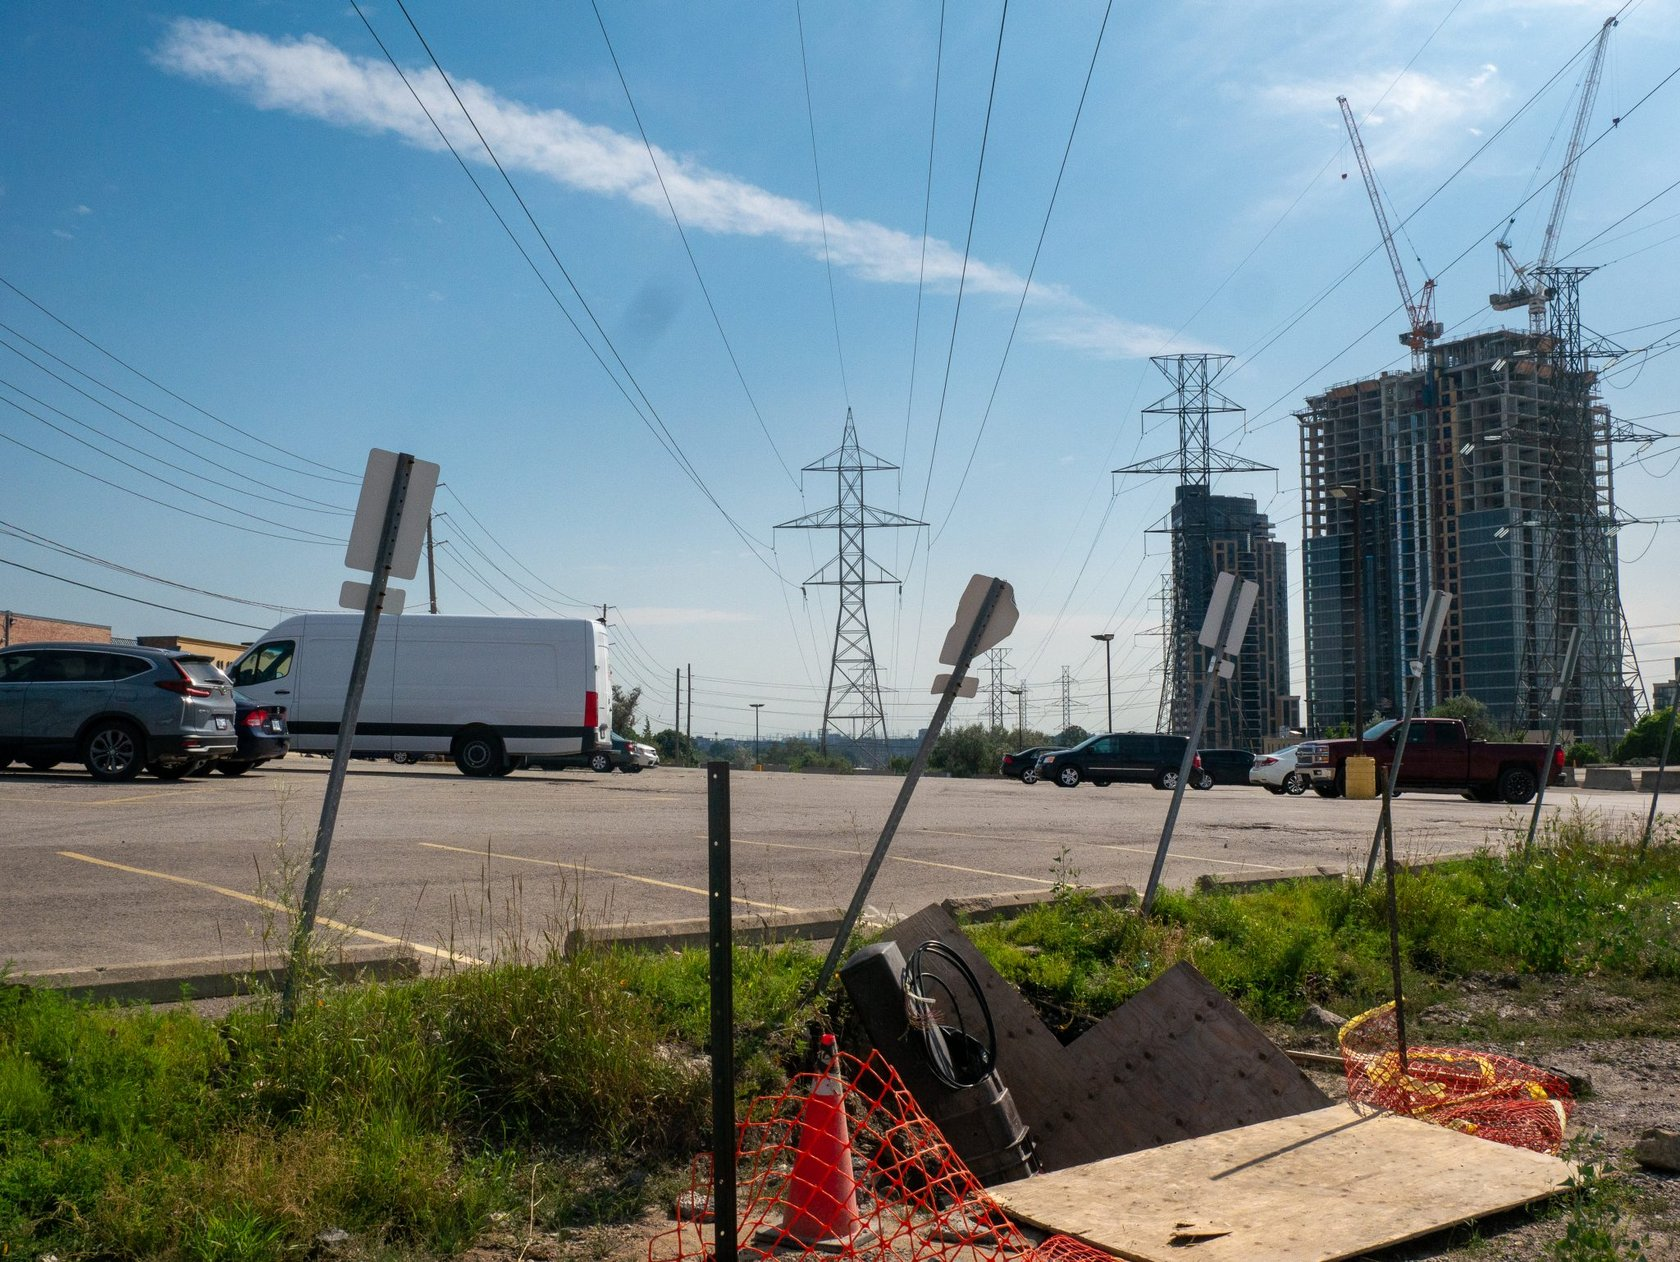
\includegraphics[width=0.7\textwidth]{images/1220594-2048x1538.jpg}
\end{figure}

The condition of the roads also had me concerned for the safety of the trishaws, the potholes, small rocks, uneven road pavement and metal sheets strewn about the roads meant that the trishaws were susceptible to many hazards. I was concerned what would happen if we were to have a tube in our Trishaw’s three tires burst from a puncture. The bumpiness of the road would also be uncomfortable for any passenger at the front!

Biking along Finch Avenue, many heads turned when they saw our trishaws. They looked perplexed or bemused by seeing such a unique three-wheeled human-powered and battery-assisted device sharing the road with vehicles.

\begin{figure}[htbp]
  \centering
  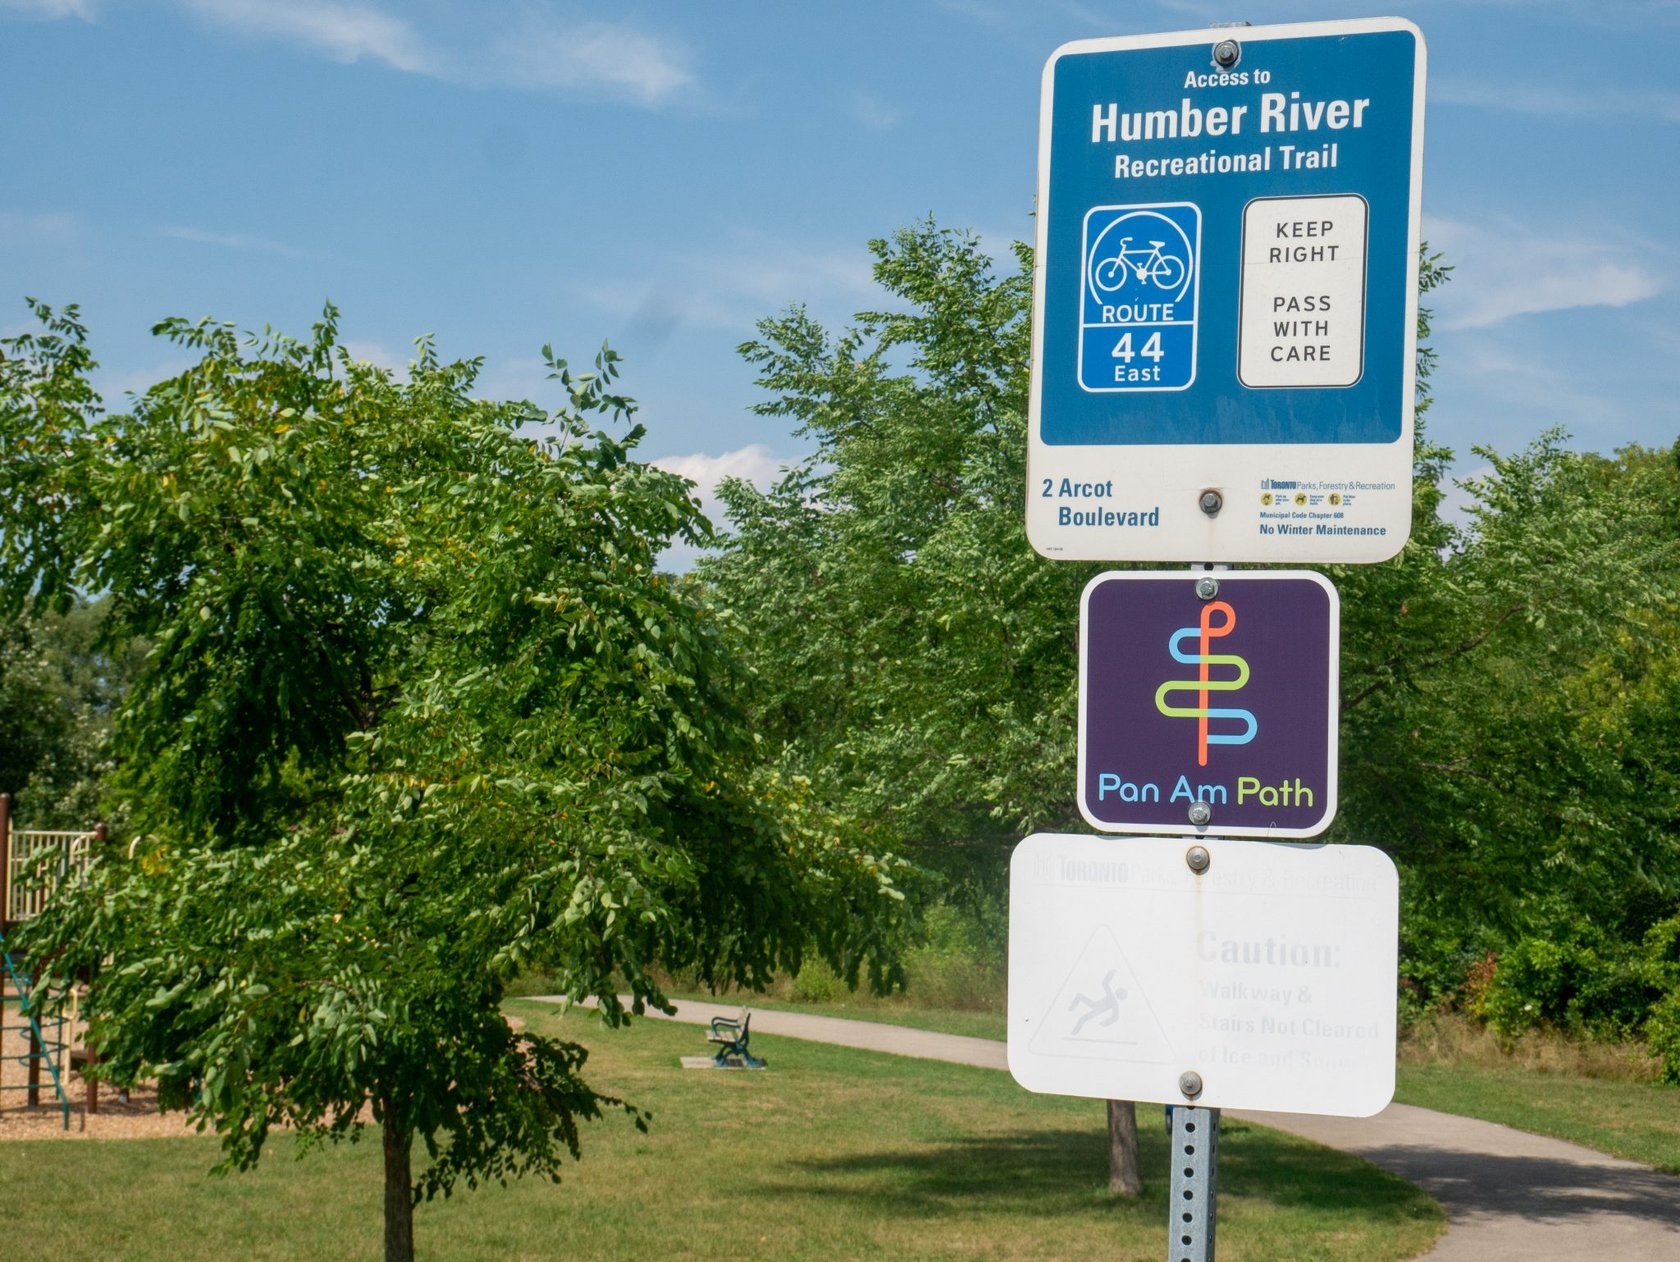
\includegraphics[width=0.7\textwidth]{images/1220563-2048x1538.jpg}
\end{figure}

While the trishaw is meant to be a comfortable, almost luxury experience, the local existing infrastructure delivered an often hostile message. Some things that would help with the trip would be wayfinding, so I can navigate my way around, and a safe space for our wider trishaws to traverse throughout Northwest Toronto’s arterial roads.

Editor’s note: Cody’s fears of a puncture were well founded. After suffering one at the corner of Finch and the 401, Cody rode our trishaw to York University on one working wheel!

\begin{figure}[htbp]
  \centering
  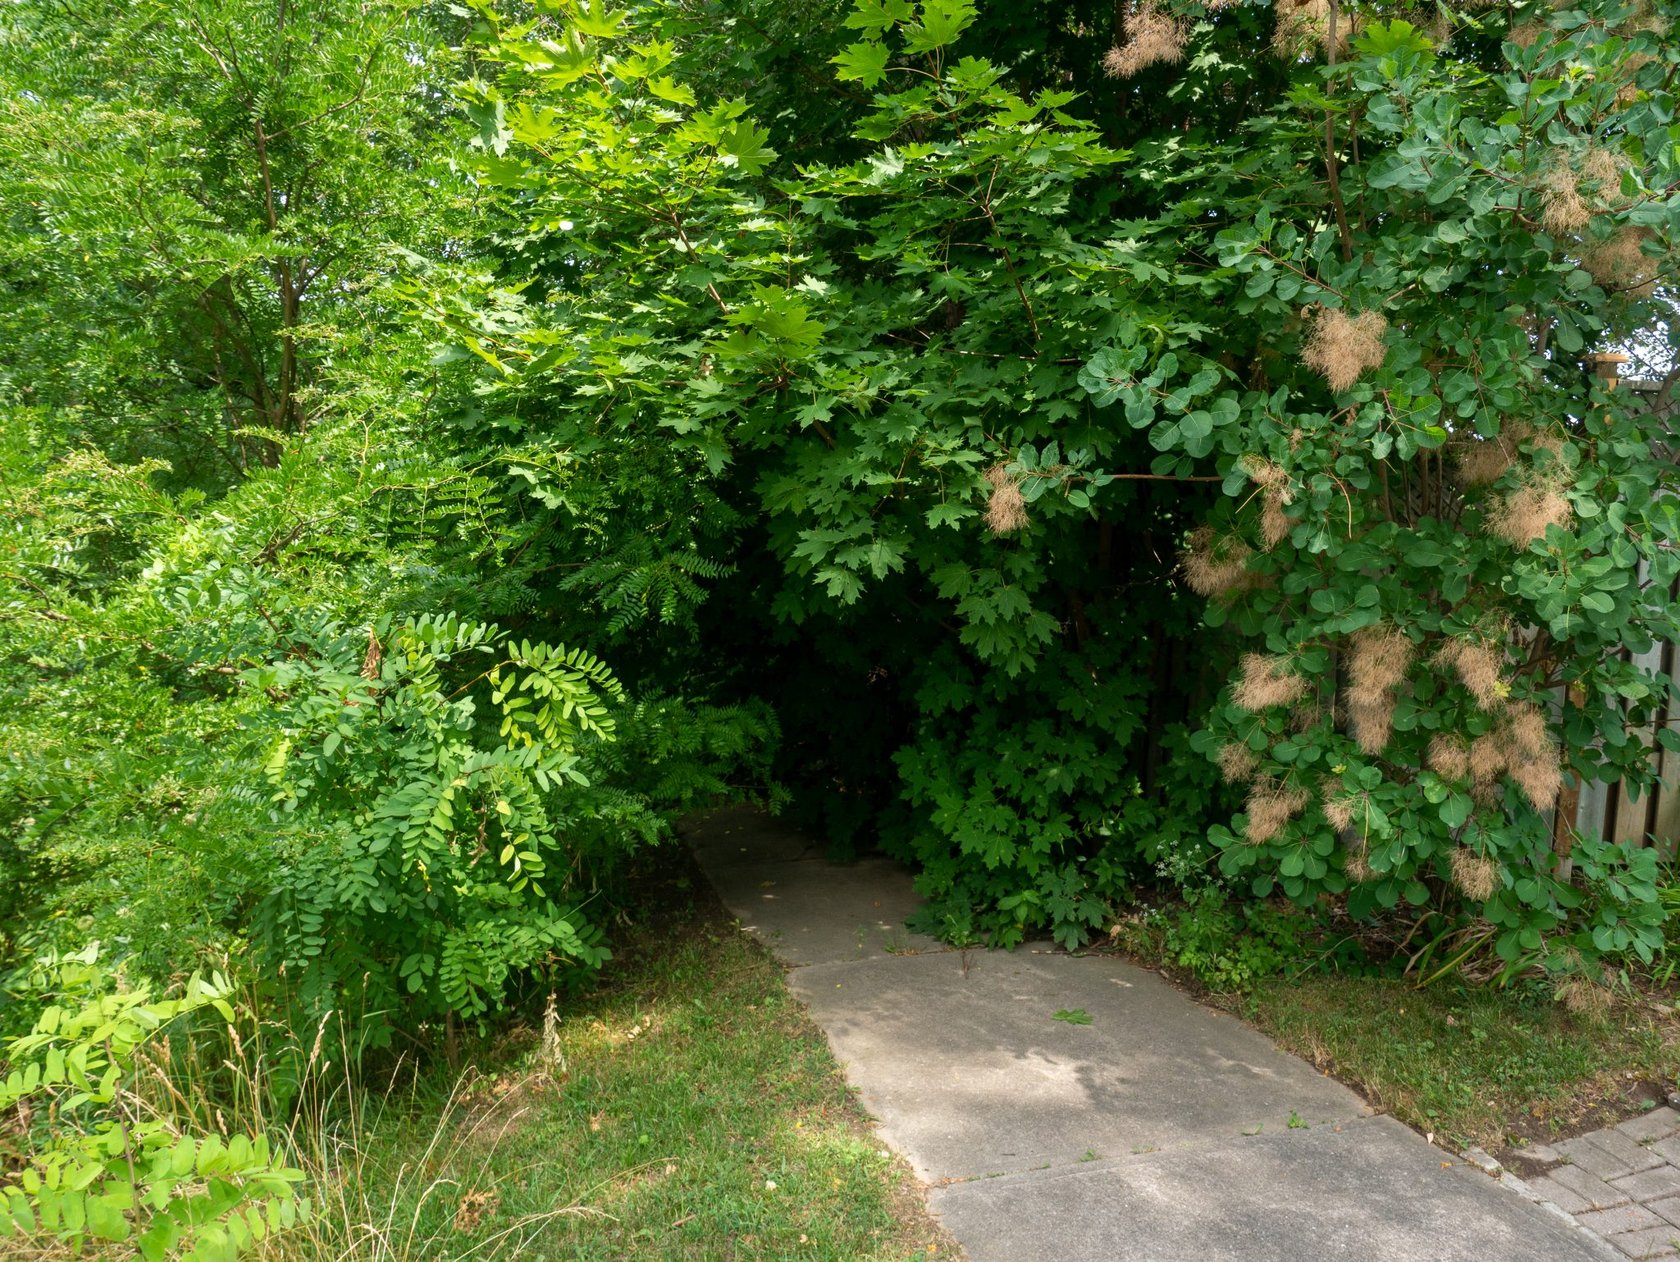
\includegraphics[width=0.7\textwidth]{images/1220507-2048x1538.jpg}
\end{figure}

\section{Francine Harris: “The Good, The Bad and The Ugly!”}
Over the years working with Our Greenway, I had heard much about hydro corridors, but until this August I had not cycled in one! So, Friday August 5th was an unforgettable day, it was my very first wheeled experience in a hydro corridor. Riding as a passenger on a trishaw, I felt excited as I listened carefully to the pilot reviewing the safety protocol for the street and hydro corridor ride.

The trip down the side streets was very interesting. As we journeyed along, I realized that viewing the private gardens, houses and trees that lined the way was so much more pleasurable at a lower level and traveling at a slower pace than being on a bus or in a car.

\begin{figure}[htbp]
  \centering
  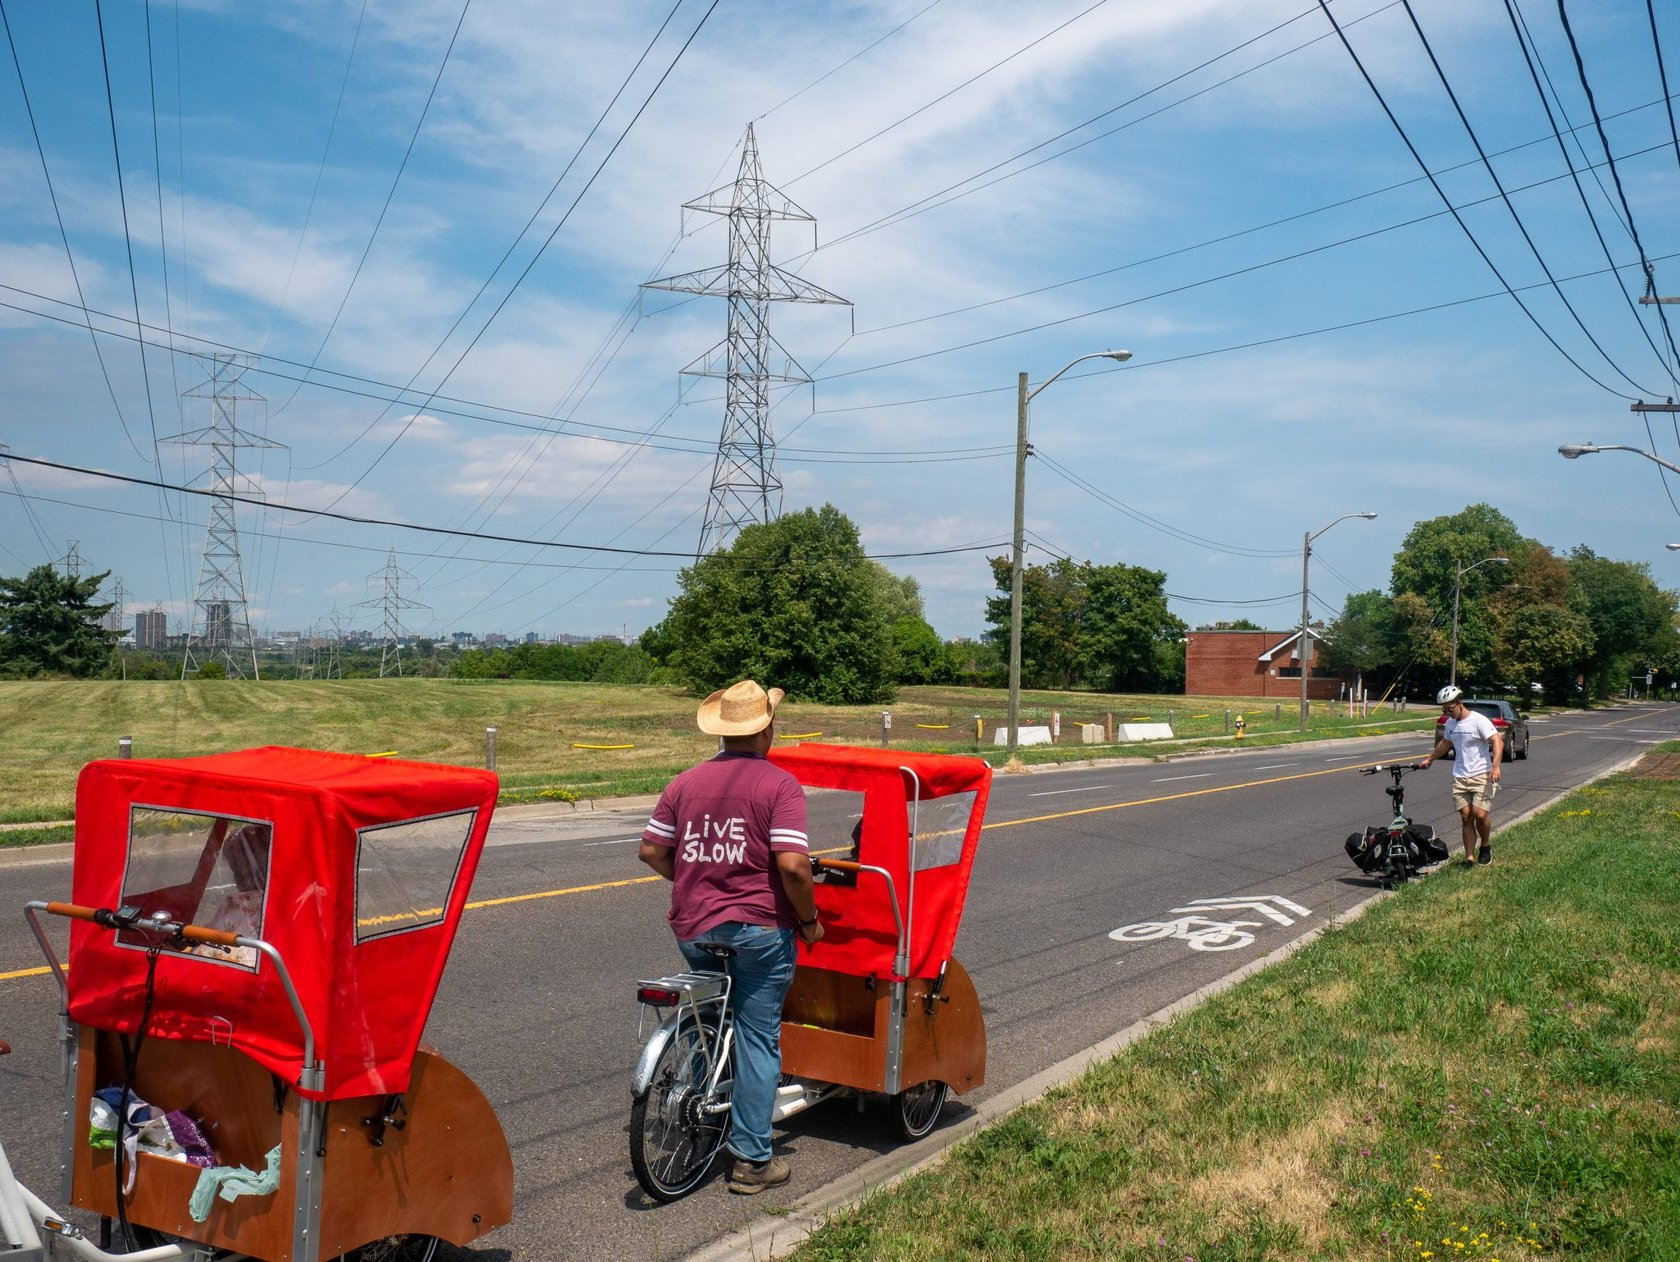
\includegraphics[width=0.7\textwidth]{images/1220518-2048x1538.jpg}
\end{figure}

The road journey was reasonably calm except when it became necessary to get onto the hydro corridor on the opposite side of the road. With some skillful maneuvering the pilot was able to arrive safely at the entrance of the hydro corridor. Five (5) of us made this journey. Two (2) e-trishaw pilots, two (2) passengers, and one (1) support  person on an e-cargo cycle.

The hydro corridor brought back many fond memories of my childhood in Dominica at Delaford, my father’s Caribbean estate. I took deep breaths filling my lungs with fresh air, whilst listening to the singing and chirping of the birds up high in the tall trees enjoying their freedom in the lush vegetation. Watching the branches, the tall wild grasses, the numerous short shrubs and wildflowers swaying gently in the breeze was so calming.

\begin{figure}[htbp]
  \centering
  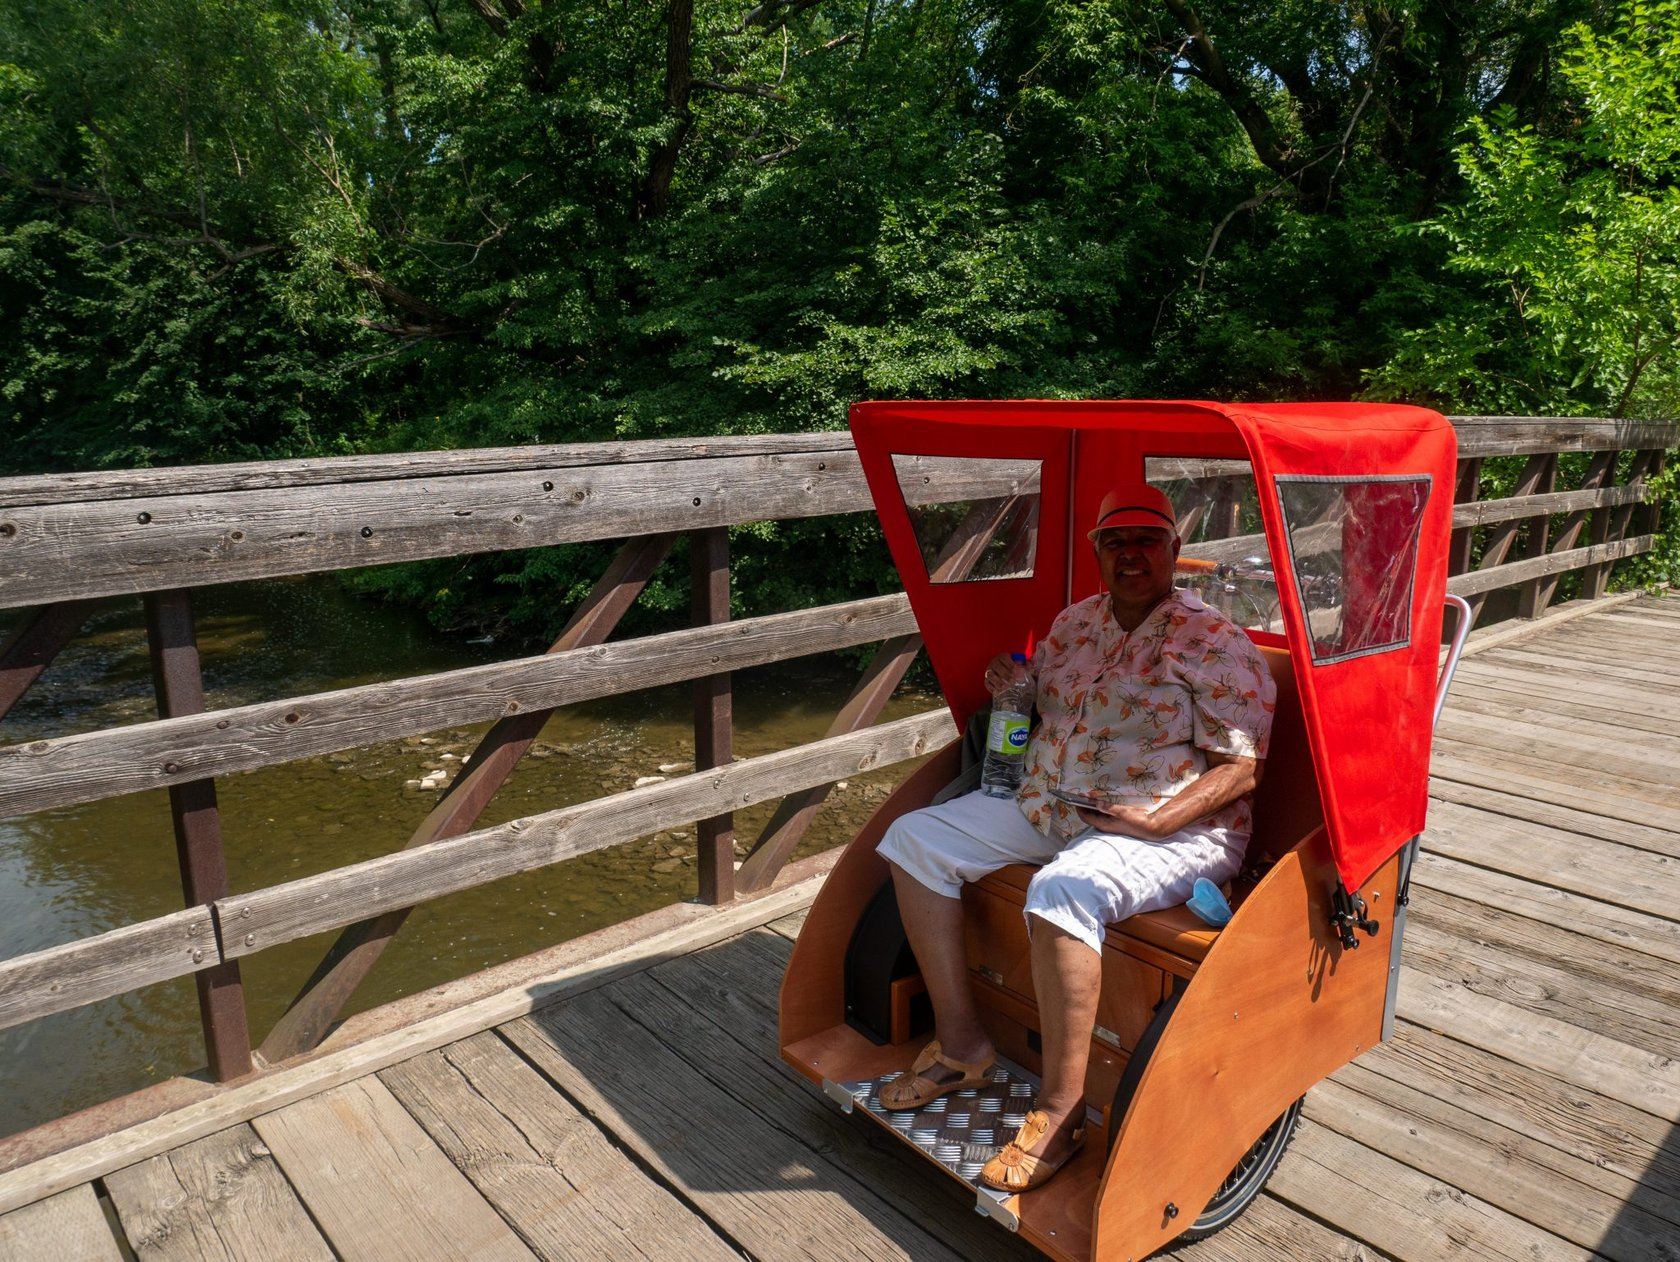
\includegraphics[width=0.7\textwidth]{images/1220575-2048x1538.jpg}
\end{figure}

We stopped along the way to take pictures of the wooden bridge, the clear bubbling stream and later the elegant herons swimming on the small pond. Experiencing this tranquility made me feel relaxed, troubles blew away even for a while.The camaraderie amongst our group of five was heart-warming. We laughed and talked on varied topics. This was infectious as we greeted walkers, joggers and bicycle riders.

Being chauffeured along the hydro corridor was truly a joy. Riding along the wide and mostly paved path felt so much more relaxing and comfortable than on the road. I saw a few worn benches, but noted the absence of garbage receptacles, restroom facilities and lighting fixtures.

\begin{figure}[htbp]
  \centering
  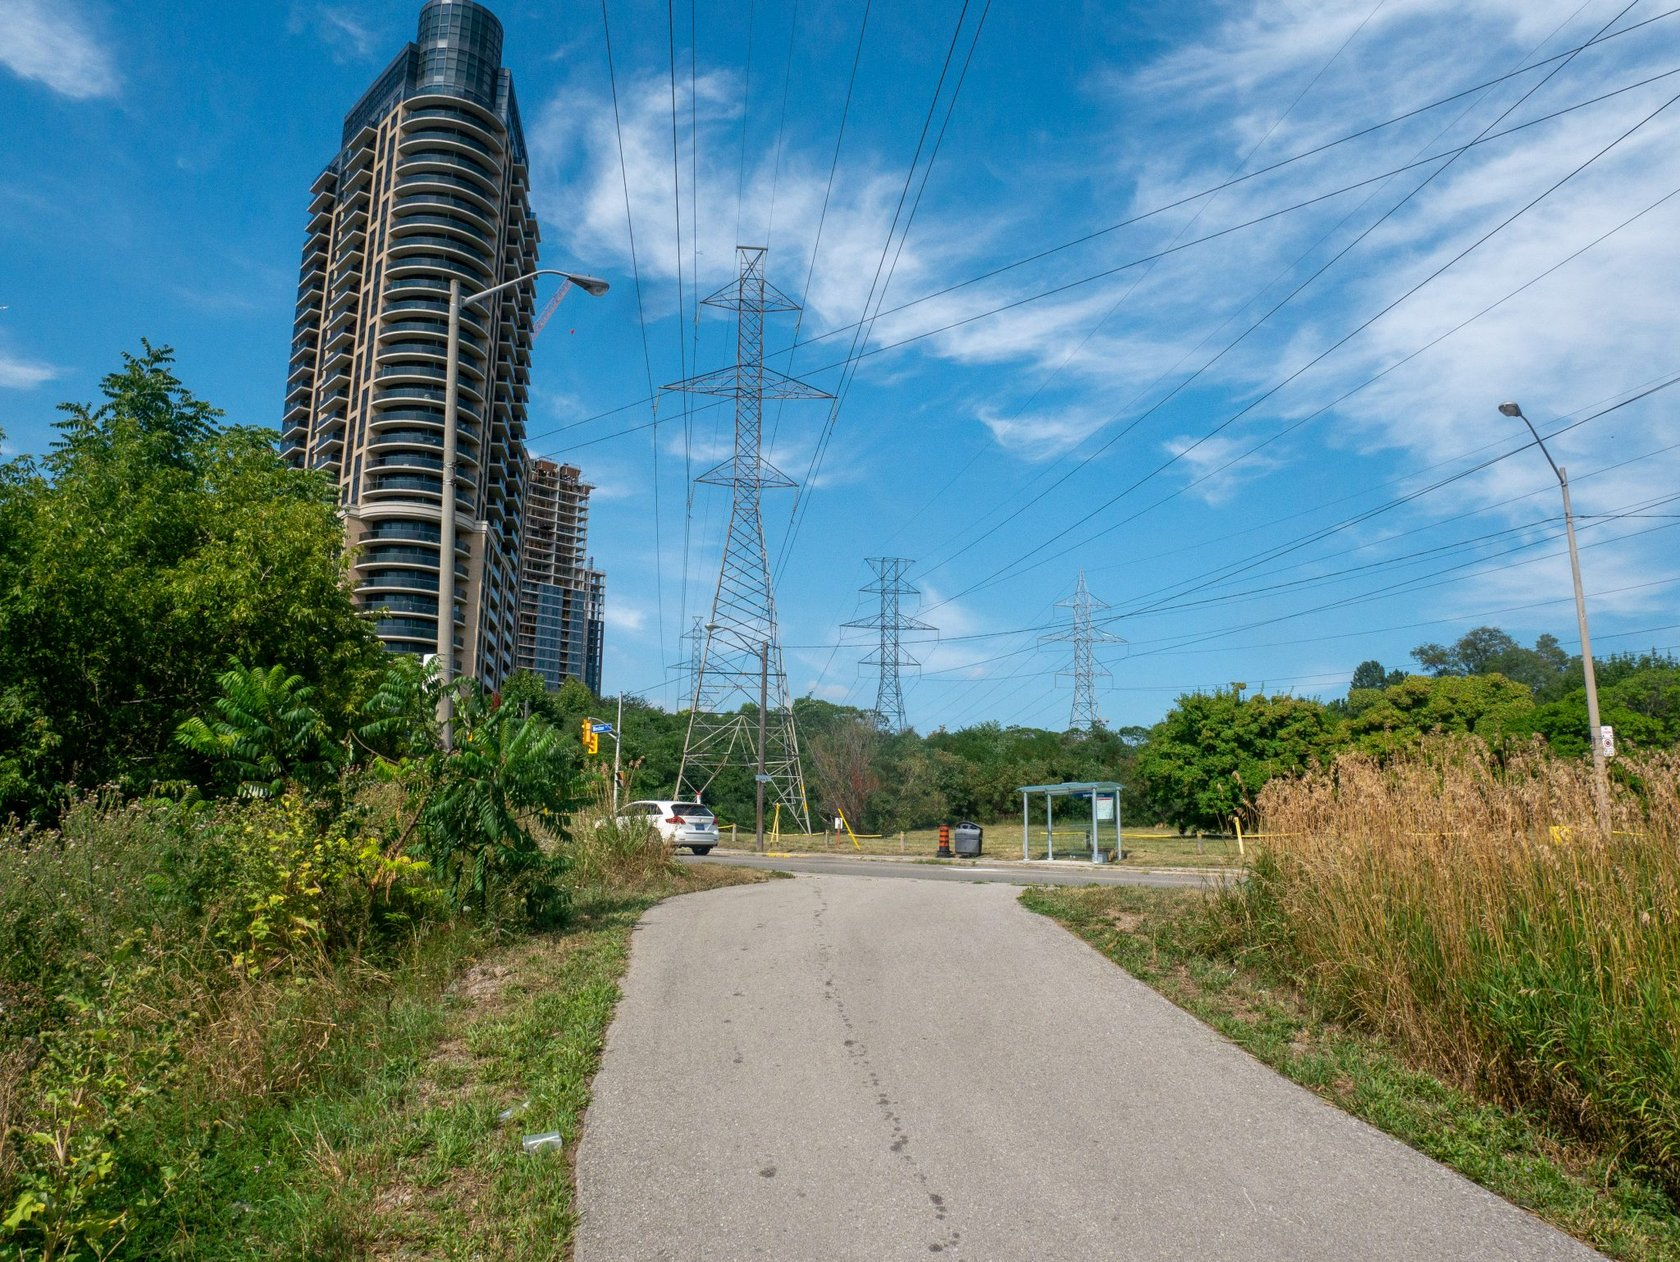
\includegraphics[width=0.7\textwidth]{images/1220586-2048x1538-1.jpg}
\end{figure}

As we neared the end of the hydro corridor, I was elated to be given the opportunity to pilot a trishaw. My happiness was short lived as I heard loud whirring noises and was told it was from the automobiles ‘flying’ down the road; that brought chills to me as I contemplated being a cyclists in such traffic.

Back onto the open street much of which was undergoing construction was extremely difficult and stressful. Automobile drivers were vying for position on the narrowed street, some drivers blew their horns despite the fact there was literally no space for passing on the 1 ½ lane opening on the road under construction.

I learned how emotionally different I felt before arriving at the hydro corridor, during the hydro corridor ride and getting back onto the busy road crowded with fast moving automobile traffic.

It was now clearer than ever how significant is the need of proper micromobility infrastructure and guidelines for the safety of all.

Editor’s note: We thank Francine for volunteering to be a passenger during the entire ride; the Finch portion was rough!

\vspace{2em}
\fbox{\parbox{\dimexpr\textwidth-2\fboxsep-2\fboxrule\relax}{
\raggedright
  \small This PDF was automatically generated using the Python-to-LaTeX tool available at~\url{https://github.com/Our-Greenway/scrape2TeX}.\\[0.5em]
  If there are any differences, the online version at~\url{https://www.ourgreenway.ca/dispatches-cwa1} shall prevail.
}}
\end{document}